\documentclass[10pt, a5paper]{article}
\usepackage{pdfpages}
\usepackage{parallel}
\usepackage[T2A]{fontenc}
\usepackage{ucs}
\usepackage[utf8x]{inputenc}
\usepackage[polish,english,russian]{babel}
\usepackage{hyperref}
\usepackage{rotating}
\usepackage[inner=2cm,top=1.8cm,outer=2cm,bottom=2.3cm,nohead]{geometry}
\usepackage{listings}
\usepackage{graphicx}
\usepackage{wrapfig}
\usepackage{longtable}
\usepackage{indentfirst}
\usepackage{array}
\newcolumntype{P}[1]{>{\raggedright\arraybackslash}p{#1}}
\frenchspacing
\usepackage{fixltx2e} %text sub- and superscripts
\usepackage{icomma} % коскі ў матэматычным рэжыме
\PreloadUnicodePage{4}

\newcommand{\longpage}{\enlargethispage{\baselineskip}}
\newcommand{\shortpage}{\enlargethispage{-\baselineskip}}

\def\switchlang#1{\expandafter\csname switchlang#1\endcsname}
\def\switchlangbe{
\let\saverefname=\refname%
\def\refname{Літаратура}%
\def\figurename{Іл.}%
}
\def\switchlangen{
\let\saverefname=\refname%
\def\refname{References}%
\def\figurename{Fig.}%
}
\def\switchlangru{
\let\saverefname=\refname%
\let\savefigurename=\figurename%
\def\refname{Литература}%
\def\figurename{Рис.}%
}

\hyphenation{admi-ni-stra-tive}
\hyphenation{ex-pe-ri-ence}
\hyphenation{fle-xi-bi-li-ty}
\hyphenation{Py-thon}
\hyphenation{ma-the-ma-ti-cal}
\hyphenation{re-ported}
\hyphenation{imp-le-menta-tions}
\hyphenation{pro-vides}
\hyphenation{en-gi-neering}
\hyphenation{com-pa-ti-bi-li-ty}
\hyphenation{im-pos-sible}
\hyphenation{desk-top}
\hyphenation{elec-tro-nic}
\hyphenation{com-pa-ny}
\hyphenation{de-ve-lop-ment}
\hyphenation{de-ve-loping}
\hyphenation{de-ve-lop}
\hyphenation{da-ta-ba-se}
\hyphenation{plat-forms}
\hyphenation{or-ga-ni-za-tion}
\hyphenation{pro-gramming}
\hyphenation{in-stru-ments}
\hyphenation{Li-nux}
\hyphenation{sour-ce}
\hyphenation{en-vi-ron-ment}
\hyphenation{Te-le-pathy}
\hyphenation{Li-nux-ov-ka}
\hyphenation{Open-BSD}
\hyphenation{Free-BSD}
\hyphenation{men-ti-on-ed}
\hyphenation{app-li-ca-tion}

\def\progref!#1!{\texttt{#1}}
\renewcommand{\arraystretch}{2} %Іначай формулы ў матрыцы зліпаюцца з лініямі
\usepackage{array}

\def\interview #1 (#2), #3, #4, #5\par{

\section[#1, #3, #4]{#1 -- #3, #4}
\def\qname{LVEE}
\def\aname{#1}
\def\q ##1\par{{\noindent \bf \qname: ##1 }\par}
\def\a{{\noindent \bf \aname: } \def\qname{L}\def\aname{#2}}
}

\def\interview* #1 (#2), #3, #4, #5\par{

\section*{#1\\{\small\rm #3, #4. #5}}

\def\qname{LVEE}
\def\aname{#1}
\def\q ##1\par{{\noindent \bf \qname: ##1 }\par}
\def\a{{\noindent \bf \aname: } \def\qname{L}\def\aname{#2}}
}



\begin{document}

\switchlang{be}
\title{Вольныя графічныя праграмы для апрацоўкі выяваў з падвышанай глыбінёй колеру}%\footnote{Текст данных и последующих тезисов, кроме специально оговоренных случаев, доступен под лицензией Creative Commons Attribution-ShareAlike 3.0}

\author{Антон Літвіненка\footnote{Кіеў, Украіна}}
\maketitle

 \begin{abstract}
  Deep color images (with more than 8 bits per channel) are supposed to be extremely useful in image processing (especially, photographic) due to better quality preservation, but are totally unsupported by GIMP. Author gives a brief overview of typical deep color processing taks and with their solutions using ufraw, ImageMagick, nip2 and Luminance HDR programs.
 \end{abstract}

Фактычным стандартам у вобласці сучаснай кампутарнай графікі з'яўляецца выкарыстанне лічбавых выяваў <<True Color>>-якасці, якая прадугледжвае выкарыстанне 8 бітаў дадзеных для перадачы значэння кожнага канала для кожнага піксела выявы. Такая колькасць інфармацыі дазваляе перадаць 256 градацый значэння кожнага канала і, ў выпадку каляровае трохканальнае выявы --- больш за 16 мільёнаў адценняў, што цалкам дастаткова для стварэння ў чалавечаскага вока ўражання натуральнага колеру. Разам з тым, пад час апрацоўкі выяваў, асабліва фатаздымкаў, інфармацыі ў <<True Color>> здымку можа апынуцца замала для атрымання настолькі ж натуральнага выніку апрацоўкі (напрыклад, калі зыходная выява фактычна выкарыстоўвае толькі частку магчымага дыяпазону колераў (надта цемная, светлая ці проста малакантрастная)). У такіх выпадках выкарыстоўваюцца разнастайныя стандарты з падвышанай <<бітнасцю>> (глыбінёй колеру), якія змяшчаюць большую колькасць градацый адценняў. Гэтыя стандарты (якія аб'ядноўваюцца пад агульнай назвай <<Deep Color>>) можна падзяліць на наступныя групы:

\begin{enumerate}
 \item сямейства фарматаў RAW (12, 14, 22 біта на канал);
 \item 16-bit (48-bit) TIFF (16 бітаў на канал);
 \item сямейства фарматаў HDR (8, 16, 32 біта на канал).
\end{enumerate}
 
Агульнавядомай адносна ўніверсальнай вольнай праграмай для інтэрактыўнай апрацоўкі выяваў з'яўляецца GIMP. У той жа час, праз прынцыповыя абмежаванні ягонай існай архітэктуры падтрымкі deep color у ім няма і бліжэйшым часам не будзе. Праз тое даводзіцца карыстацца альбо праграмамі, адмыслова прызначанымі для пэўных аспектаў deep color апрацоўкі (ufraw, Luminance HDR), альбо прыстасоўваць праграмы, прызначаныя, ў прынцыпе, для іншых мэтаў (ImageMagick, nip2).

\section*{Апрацоўка RAW}

RAW --- нестандартызаванае сямейства фарматаў, прызначаных для захоўвання выяваў з лічбавых фотакамер з мінімальнай апрацоўкай працэсарам камеры. Дазваляе захаваць максімальную колькасць першаснай інфармацыі для ёйнай апрацоўкі па-за межамі сэансу фатаграфавання. Праз вялікую колькасць варыянтаў фармату, незваротнасць апрацоўкі (у RAW не захоўваюць пасля апрацоўкі), а таксама праз спецыфічныя аперацыі (баераўскі фільтр, накладанне балансу белага і г.д.) апрацоўка RAW выконваецца адмысловымі праграмамі альбо адмысловымі плагінамі. FLOSS- \linebreak прыкладам з'яўляецца \textbf{ufraw}, які існуе як у выглядзе плагіна для GIMP, так і ў выглядзе асобнае праграмы (можа ствараць 48-бітныя TIFF-файлы для дадатковай апрацоўкі, калі гэта патрэбна). Праграма цалкам рэалізуе <<праяўленне>> RAW-выявы разам з шэрагам дадатковых спецыфічных для фотаздымкаў апрацовак (карэкцыя неідэальнасці лінзаў, застасаванне <<чорнага кадру>> (карэкцыя бітых пікселаў), вэйвлетнае падаўленне шумоў і г.д.).

Зручна паядноўваць выкарыстанне ufraw з выкарыстаннем праграмаў, здольных да хуткага папярэдняга прагляду RAW.

Іншыя варыянты: \textbf{darktable}, \textbf{rawstudio}.

%http://summer.lvee.org/uploads/abstract_file/file/30/LAS_LVEE_2012_RAW.jpg
\begin{figure}[htpb]
\centering
 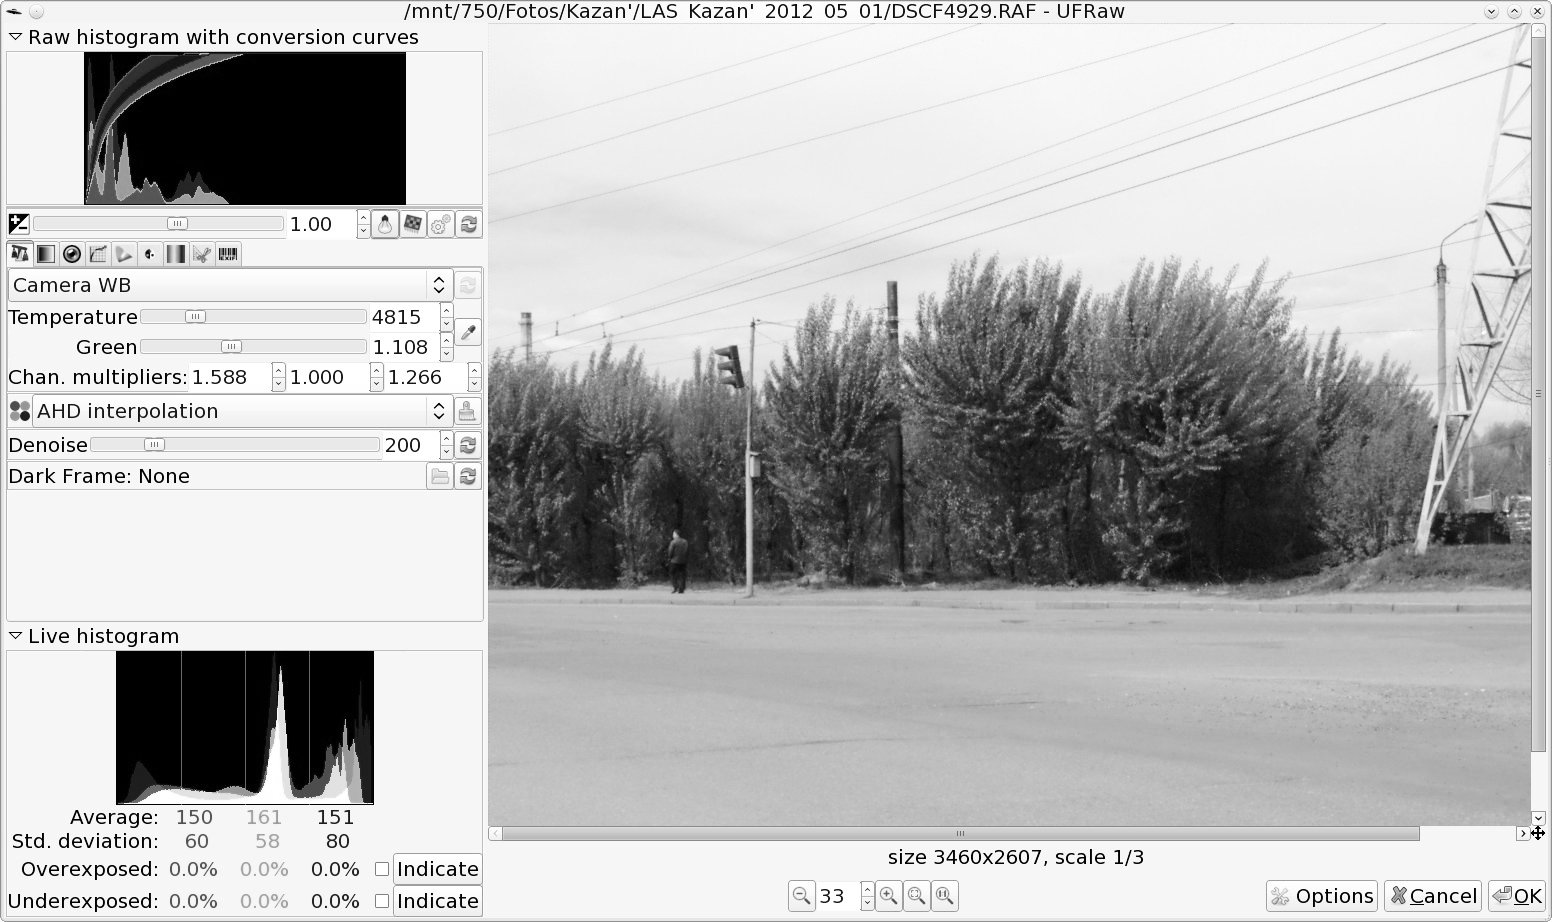
\includegraphics[width=85mm]{LAS_LVEE_2012_RAW_gs.jpg}
 \caption{RAW-файл у вакне праграмы ufraw}
 \label{fig:RAW}
\end{figure}

\section*{Апрацоўка HDR}

HDR-выявы таксама з'ўляюцца спецыфічным выпадкам deep color выяваў, галоўная мэта якога --- перадаць вялікі дынамічны дыяпазон адлюстраванае сцэны. Стварэнне такіх выяваў ускладненае абмежаванасцю:
\begin{enumerate}
 \item  Фатаапаратаў (замалы дынамічны дыяпазон сенсара);
\item  Фарматаў захоўвання (могуць змяшчаць замалы дынамічны дыяпазон);
\item  Тэхнікі для адлюстравання (дысплей, фотапапера).
\end{enumerate}
Рашэнне --- застасаванне спецыфічных спосабаў на ўсіх этапах:
\begin{enumerate}
\item  Стварэнне: аб'яднанне некалькіх LDR выяваў;
\item  Захоўванне: адмысловыя фарматы;
\item  Адлюстраванне: пераўтварэнне ў LDR выяву асаблівымі адаптыўнымі алгарытмамі (tonemapping).
\end{enumerate}

Прыклад FLOSS-праграмы: \textbf{Luminance HDR}.

Магчыма захаванне 48-бітнай выявы і далейшая апрацоўка (рэзультат працы tonemapping-алгарытмаў не заўсёды аптымальны, і часам мэтазгодна застасаваць далейшую карэкцыю).

\section*{Рэдагаванне класічных 48-бітных выяваў}

Аб'екты:
\begin{enumerate}
\item сканаваныя плёнкі;
\item фатаздымкі у фармаце 48-bit TIFF;
\item фатаздымкі пасля папярэдняй RAW- ці HDR-апрацоўкі.
\end{enumerate}
Тыповыя задачы:
\begin{enumerate}
\item Змена баланса белага (паканальная змена яркасці);
\item Рэдагаванне яркасці/кантрасту праз узроўні і гамму (чорны, белы, шэры пункты);
\item Рэдагаванне яркасці/кантрасту праз іншыя функцыі \linebreak (напрыклад,  сігмаідальны кантраст).
\end{enumerate}
Усе задачы зводзяцца да аперацыяў з колерам (застасаванне пэўных функцыяў да значэнняў ўсіх пікселаў выявы). Геаметрычныя аперацыі мэтазгодна рабіць з канчатковай True Color выявай.

\textbf{ImageMagick} --- праграма для пакетнай апрацоўкі выяваў.

Прыклады застасавання для апрацоўкі сканаванае выявы:
\begin{itemize}
 \item Прыглушэнне сіняга каналу сканаванага слайда:

 \texttt{convert 1.tif -channel blue -gamma 0.95 2.tif}

\item Павялічэнне яркасці ды кантрастнасці --- варыянт 1:

 \texttt{convert 2.tif -level 5\%,100\%,1.2 3.tif}

\item Павялічэнне яркасці ды кантрастнасці --- варыянт 2:

 \texttt{convert 2.tif -sigmoidal-contrast 2.5,35\% 4.tif}

\end{itemize}

\textbf{Nip2} --- праграма, аптымізаваная для апрацоўкі вялікіх выяваў. Прынцып працы нагадвае электронную табліцу (задаецца паслядоўнасць фільтраў, каторыя застасоўваюцца да пікселяў, рыс.~\ref{fig:nip2}).

Выкарыстанне абодвух праграмаў павязанае са зменай звычнага стылю рэдагавання выяваў і патрабуе некаторага звыкання.

\begin{figure}[htpb]
\centering
 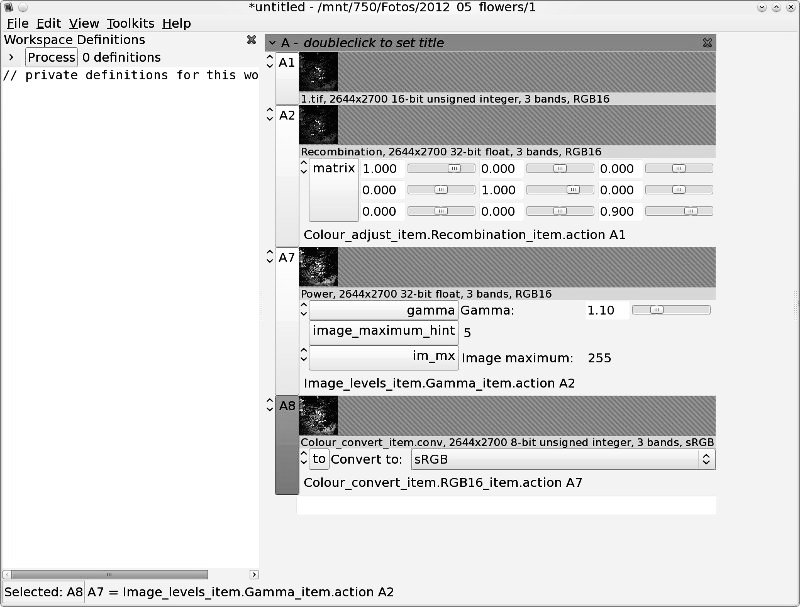
\includegraphics[width=85mm]{LAS_LVEE_2012_nip2_gs.jpg}
 \caption{Апрацоўка выявы ў вакне праграмы nip2}
 \label{fig:nip2}
\end{figure}
Такім чынам, выкарыстанне выяваў з падвышанай глыбінёй колеру з'яўляецца важлівым для пытанняў апрацоўкі выяваў, асабліва фатаздымкаў. З-за праблем з падтрымкай deep color выяваў інтэрактыўнмi рэдактарамi тыпу GIMP, атрымліваецца застасаваць іншыя праграмы, пачаткова не прызначаныя для гэтае мэты.
\end{document}

